\documentclass[11pt]{article}
\usepackage[a4paper,total={6in,9.5in}]{geometry}

\usepackage{textcomp}
\usepackage{tikz}
\usepackage{amsmath}
\usepackage{amsfonts}
\usepackage{amssymb}

\usepackage{booktabs}
\usepackage{makecell}
\usepackage{caption}
\DeclareCaptionFont{xipt}{\sffamily}
\usepackage[font=xipt, labelfont=bf]{caption}
\usepackage{subcaption}

\usepackage{enumitem}
\usepackage{setspace}
\usepackage{etoolbox}
\AtBeginEnvironment{quote}{\par\singlespacing\small}

\usepackage{graphicx}
    \graphicspath{{images/}}

\usepackage{tcolorbox}
\usepackage{thmtools}
\tcbuselibrary{theorems}
\newtcbtheorem[number within=section]{theorem}{Theorem}%
    {colback=white!15,colframe=black,fonttitle=\bfseries,arc=0pt,outer arc=0pt}{th}
\newtcbtheorem[number within=section]{definition}{Definition}%
    {colback=white!15,colframe=black,fonttitle=\bfseries,arc=0pt,outer arc=0pt}{th}

\usepackage[backend=bibtex]{biblatex}
\addbibresource{references.bib}

\newcommand{\AP}{AP\textsuperscript{\small\textregistered} }
\newcommand{\pr}{\mathop{\mathbf{Pr}}}
\newcommand{\ev}{\mathop{\mathbf{E}}}
\newcommand{\var}{\mathop{\mathrm{Var}}}

\title{Notes for \AP Statistics Exam}
\author{Yuanqi Li\\Humble Academy, Nanjing}
\date{}

\begin{document}

\maketitle
\tableofcontents
\clearpage

% \section{About \AP Statistics Exam}

% \section{Exploring One-Variable Data}

% \section{Exploring Two-Variable Data}

\subsection{Unit Guide}

\subsubsection{Developing Understanding}

Building on Unit 1, students will explore relationships in two-variable categorical or quantitative data sets. They will use graphical and numerical methods to investigate an association between two categorical variables. Skills learned while working with two-way tables will transfer to calculating probabilities in Unit 4.

Students will describe form, direction, strength, and unusual features for an association between two quantitative variables. They will assess correlation and, if appropriate, use a linear model to predict values of the response variable from values of the explanatory variable. Students will interpret the least-squares regression line in context, analyze prediction errors (residuals), and explore departures from a linear pattern.

\subsubsection{Building Course Skills}

In Unit 2, students are looking at the relationship between variables. The ability to calculate and describe statistical values, such as a conditional relative frequency or the slope of a regression line, is critical for data analysis because students must be able to analyze patterns before drawing conclusions about the data. Students should be allowed to perform their calculations using technology to help them become more aware of procedural errors. Students will also need practice translating output from technology (``calculator speak'') into appropriate statistical language.

As any statistician will assert, a numerical calculation is only as good as one's ability to interpret what it means in the real world. Rather than just reporting values from their calculations, students must be able to connect their numerical results to the scenario's context and formulate a verbal response that makes that connection clear. Teachers can model good communication and provide high-quality feedback to help students use accurate statistical language when comparing side-by-side bar graphs, for example, and to avoid common errors in reasoning, such as using the word ``line'' to explain why a relationship is linear.

\subsubsection{Preparing for the AP Exam}

Students need ongoing practice with interpretation of vocabulary and calculated values in context. It is typically not sufficient to speak generally about the direction of a relationship, for example. If the question is about a linear model for predicting the weight of a wolf based on its length, students should write that a positive relationship means that longer wolves tend to have higher weights (see 2017 FRQ 1). Students can communicate statistical uncertainty by using words such as ``tend to have'' and ``on average,'' being careful to be precise with language. For example, when explaining evidence of a linear relationship, the difference between discussing a rate of change, as opposed to a change, is the difference between right and wrong. For the sake of clarity, the word ``correlation'' should be reserved for discussions about relationships between two quantitative variables.

\subsection{Least-Squares Regression}

A \textbf{regression line} is a line that describes how a response variable $y$ changes as an explanatory variable $x$ changes. We often use a regression line to predict the value of $y$ for a given value of $x$.

Suppose that $y$ is a response variable and $x$ is an explanatory variable. A regression line relating $y$ to $x$ has an equation of the form
\[
    \hat{y} = a + bx,
\]
where
\begin{itemize}[itemsep=0pt]
\item $\hat{y}$ is the \textbf{predicted value} of the response variable $y$ for a given value of the explanatory variable $x$.
\item $b$ is the \textbf{slope}, the amount by which $y$ is the predicted to change when $x$ increases by one unit.
\item $a$ is the \textbf{$\mathbf{y}$-intercept}, the predicted value of $y$ when $x = 0$.
\end{itemize}



\section{Describing Relationships}

\subsection{Scatterplots}

A \textbf{scatterplot} displays the relationship between two quantitative variables measured on the same individuals. Mark values of one variable on the horizontal axis ($x$-axis) and values of the other variable on the vertical axis ($y$-axis). Plot each individual's data as a point on the graph.

\begin{definition}{Scatterplot}{}
    A \textbf{scatterplot} shows the relationship between two quantitative variables measured on the same individuals. The values of one variable appear on the horizontal axis, and the values of the other variable appear on the vertical axis. Each individual in the data appears as a point in the graph.
\end{definition}

If we think that a variable $x$ may help explain, predict, or even cause changes in another variable $y$, we call $x$ an \textbf{explanatory variable} and $y$ a \textbf{response variable}. Always plot the explanatory variable, if there is one, on the $x$ axis of a scatterplot. Plot the response variable on the $y$ axis. If there is no explanatory-response distinction, either variable can go on the horizontal axis.

In examining a scatterplot, look for an overall pattern showing the \textbf{direction}, \textbf{form}, and \textbf{strength} of the relationship and then look for \textbf{outliers} or other departures from this pattern.

\begin{itemize}[font=\sffamily\bfseries, leftmargin=1.95cm, style=nextline, itemsep=0cm]
\item[Direction] If the relationship has a clear direction, we speak of either \textit{positive association} or \textit{negative association}.
\item[Form] \textit{Linear relationships}, where the points show a straight-line pattern, are an important form of relationship between two variables. \textit{Curved relationships} and clusters are other forms to watch for.
\item[Strength] The strength of a relationship is determined by \textit{how close} the points in the scatterplot lie to a simple form such as a line.
\end{itemize}

\subsection{Correlation}

The \textbf{correlation} $r \in [-1, +1]$ measures the \textit{strength} and \textit{direction} of the \textit{linear association} between two quantitative variables $x$ and $y$. Although you can calculate a correlation for \textit{any} scatterplot, $r$ measures strength for \textit{only} straight-line relationships.

Correlation indicates the direction of a linear relationship by its sign and magnitude:

\begin{itemize}[itemsep=0cm]
\item $r > 0$ for a positive association;
\item $r < 0$ for a negative association;
\item $r = \pm 1$ occurs only when the points on a scatterplot lie exactly on a straight line; and
\item $|r|$ indicates the strength of a linear relationship by how close it is to -1 or +1.
\end{itemize}

\begin{definition}{Correlation}{}
    The \textbf{correlation} $r$ measures the direction and strength of the linear relationship between two quantitative variables. \\
    Suppose that we have data on variables $x$ and $y$ for $n$ individuals given as:
    \[
        (x_1, y_1), (x_2, y_2), ..., (x_n, y_n).
    \]
    The means and standard deviations of the two variables are $\bar{x}$ and $s_x$ for the $x$-values, and $\bar{y}$ and $s_y$ for the $y$-values. The correlation $r$ between $x$ and $y$ is given by
    \begin{align*}
        r
        = \dfrac{1}{n-1} \sum_{i=1}^{n}
            \left( \dfrac{x_i - \bar{x}}{s_x} \right)
            \left( \dfrac{y_i - \bar{y}}{s_y} \right)
        = \dfrac{1}{n-1} \sum_{i=1}^{n} z_{x_i} z_{y_i}.
    \end{align*}
\end{definition}

\begin{figure}[ht!]
    \centering
    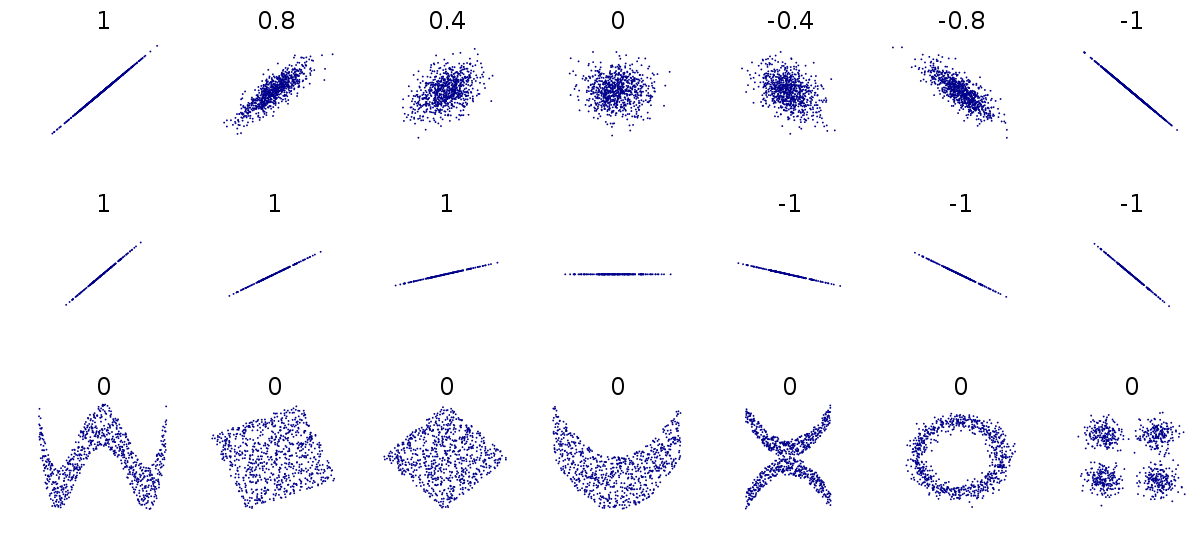
\includegraphics[width=\linewidth]{ch03/correlation.png}
    \caption{Several sets of $(x, y)$ points, with the correlation coefficient of $x$ and $y$ for each set. The correlation reflects the noisiness and direction of a linear relationship (top row), but not the slope of that relationship (middle), nor many aspects of nonlinear relationships (bottom). N.B.: the figure in the center has a slope of 0 but in that case the correlation coefficient is undefined because the variance of $y$'s is zero.}
\end{figure}

How correlation behaves is more important than the details of the formula. Here's what you need to know in order to interpret correlation correctly.

\begin{itemize}[itemsep=0cm]
\item Correlation makes no distinction between explanatory and response variables.
\item Because $r$ uses the standardized values of the observations, $r$ does not change when we change the units of measurement of $x$, $y$, or both.
\item The correlation $r$ itself has no unit of measurement.
\end{itemize}

Describing the relationship between two variables is more complex than describing the distribution of one variable. Here are some cautions to keep in mind when you use correlation.

\begin{itemize}[itemsep=0cm]
\item Correlation does not imply causation.
\item Correlation requires that both variables be quantitative, so that it makes sense to do the arithmetic indicated by the formula for $r$.
\item Correlation only measures the strength of a \textit{linear relationship} between two variables, i.e., it does not describe \textit{curved relationships} between variables, no matter how strong the relationship is.
\item A value of $r$ close to $1$ or $-1$ does not guarantee a linear relationship between two variables, e.g., when the underlying relationship is curved but not linear.
\item Like mean and standard deviation, the correlation is not resistant: $r$ is strongly affected by a few outlying observations. Use $r$ with caution when outliers appear in the scatterplot.
\item Correlation is not a complete summary of two-variable data, even when the relationship between the variables is linear. You should give the means and standard deviations of both $x$ and $y$ along with the correlation.
\end{itemize}

\subsection{Linear Regression}

A \textbf{regression} line is a \textit{model} for the data. It summarizes the relationship between two variables, but only in a specific setting: when one of the variables helps explain or predict the other. Regression, unlike correlation, requires that we have an explanatory variable and a response variable.

\begin{definition}{Regression line}{}
    A \textbf{regression line} is a line that describes how a response variable $y$ changes as an explanatory variable $x$ changes. We often use a regression line to predict the value of $y$ for a given value of $x$. \\
    Suppose that $y$ is a response variable (plotted on the vertical axis) and $x$ is an explanatory variable (plotted on the horizontal axis). A regression line relating $y$ to $x$ has an equation of the form
    \[
        \hat{y} = a + bx,
    \]
    where
    \begin{itemize}[itemsep=0cm]
    \item $\hat{y}$ (read ``$y$ hat'') is the \textbf{predicted value} of the response variable $y$ for a given value of the explanatory variable $x$;
    \item $b$ is the \textbf{slope}, the amount by which $y$ is predicted to change when $x$ increases by one unit; and
    \item $a$ is the \textbf{$\mathbf{y}$-intercept} the predicted value of $y$ when $x = 0$.
    \end{itemize}
\end{definition}
Few relationships are linear for \textit{all} values of the explanatory variable. Don't make predictions using values of $x$ that are \textit{much larger} or \textit{much smaller} than those that actually appear in your data.

A good regression line makes the vertical deviations of the points from the line as small as possible. These vertical deviations represent ``leftover'' variation in the response variable after fitting the regression line. For that reason, they are called \textbf{residuals}.

\begin{definition}{Residual}{}
    A \textbf{residual} is the difference between an observed value of the response variable and the value predicted by the regression line, i.e.,
    \begin{align*}
        \text{residual}
        &= \text{observed $y$} - \text{predicted $y$} \\
        &= y - \hat{y}.
    \end{align*}
\end{definition}

The regression line we want is the one that minimizes the sum of the squared residuals.

\begin{definition}{Least-squares regression line}{}
    The \textbf{least-squares regression line} of $y$ on $x$ is the line that makes the sum of the squared residuals as small as possible.\\
    Suppose that we have data on variables $x$ and $y$ for $n$ individuals given as:
    \[
        (x_1, y_1), (x_2, y_2), ..., (x_n, y_n).
    \]
    The means and standard deviations of the two variables are $\bar{x}$ and $s_x$ for the $x$-values, and $\bar{y}$ and $s_y$ for the $y$-values. The least-squares regression line is the line $\hat{y} = a + bx$ where
    \[
        b = r \dfrac{s_y}{s_x} \quad\text{and}\quad
        a = \bar{y} - b \bar{x}.
    \]
\end{definition}

Note that when displaying the equation of a least-squares regression line, the calculator will report the slope and intercept with much more precision than we need. However, there is no firm rule for how many decimal places to show for answers on the AP exam. The advice is that decide how much to round based on the context of the problem you are working on.

Although residuals can be calculated from any model that is fitted to the data, the residuals from the least-squares line have a special property: the mean of the least-squares residuals is \textit{always} zero.

Correlation and regression are powerful tools for describing the relationship between two variables. When you use these tools, you should be aware of their limitations.

\begin{itemize}[itemsep=0cm]
\item The distinction between explanatory and response variables is important in regression.
\item Correlation and regression lines describe only linear relationships, i.e., the results are useful only if the scatterplot shows a linear pattern. Always plot your data. See also Figure \ref{fig:anscombe}.
\item Correlation and least-squares regression lines are not resistant. One unusual point in a scatterplot can greatly change the value of $r$. Least-squares lines make the sum of the squares of the vertical distances to the points as small as possible. A point that is extreme in the $x$ direction with no other points near it pulls the line toward itself. We call such points \textbf{influential}. See also Figure \ref{fig:anscombe} and \ref{fig:regression-outlier}.
\item Association does not imply causation. A strong association between two variables is not enough to draw conclusions about cause and effect.
\end{itemize}

\begin{definition}{Outliers and influential observations in regression}{}
    An \textbf{outlier} is an observation that lies outside the overall pattern of the other observations. Points that are outliers in the $y$ direction but not the $x$ direction of a scatterplot have large residuals. Other outliers may not have large residuals. \\
    An observation is \textbf{influential} for a statistical calculation if removing it would markedly change the result of the calculation. Points that are outliers in the $x$ direction of a scatterplot are often influential for the least-squares regression line.
\end{definition}

\begin{figure}[ht!]
    \centering
    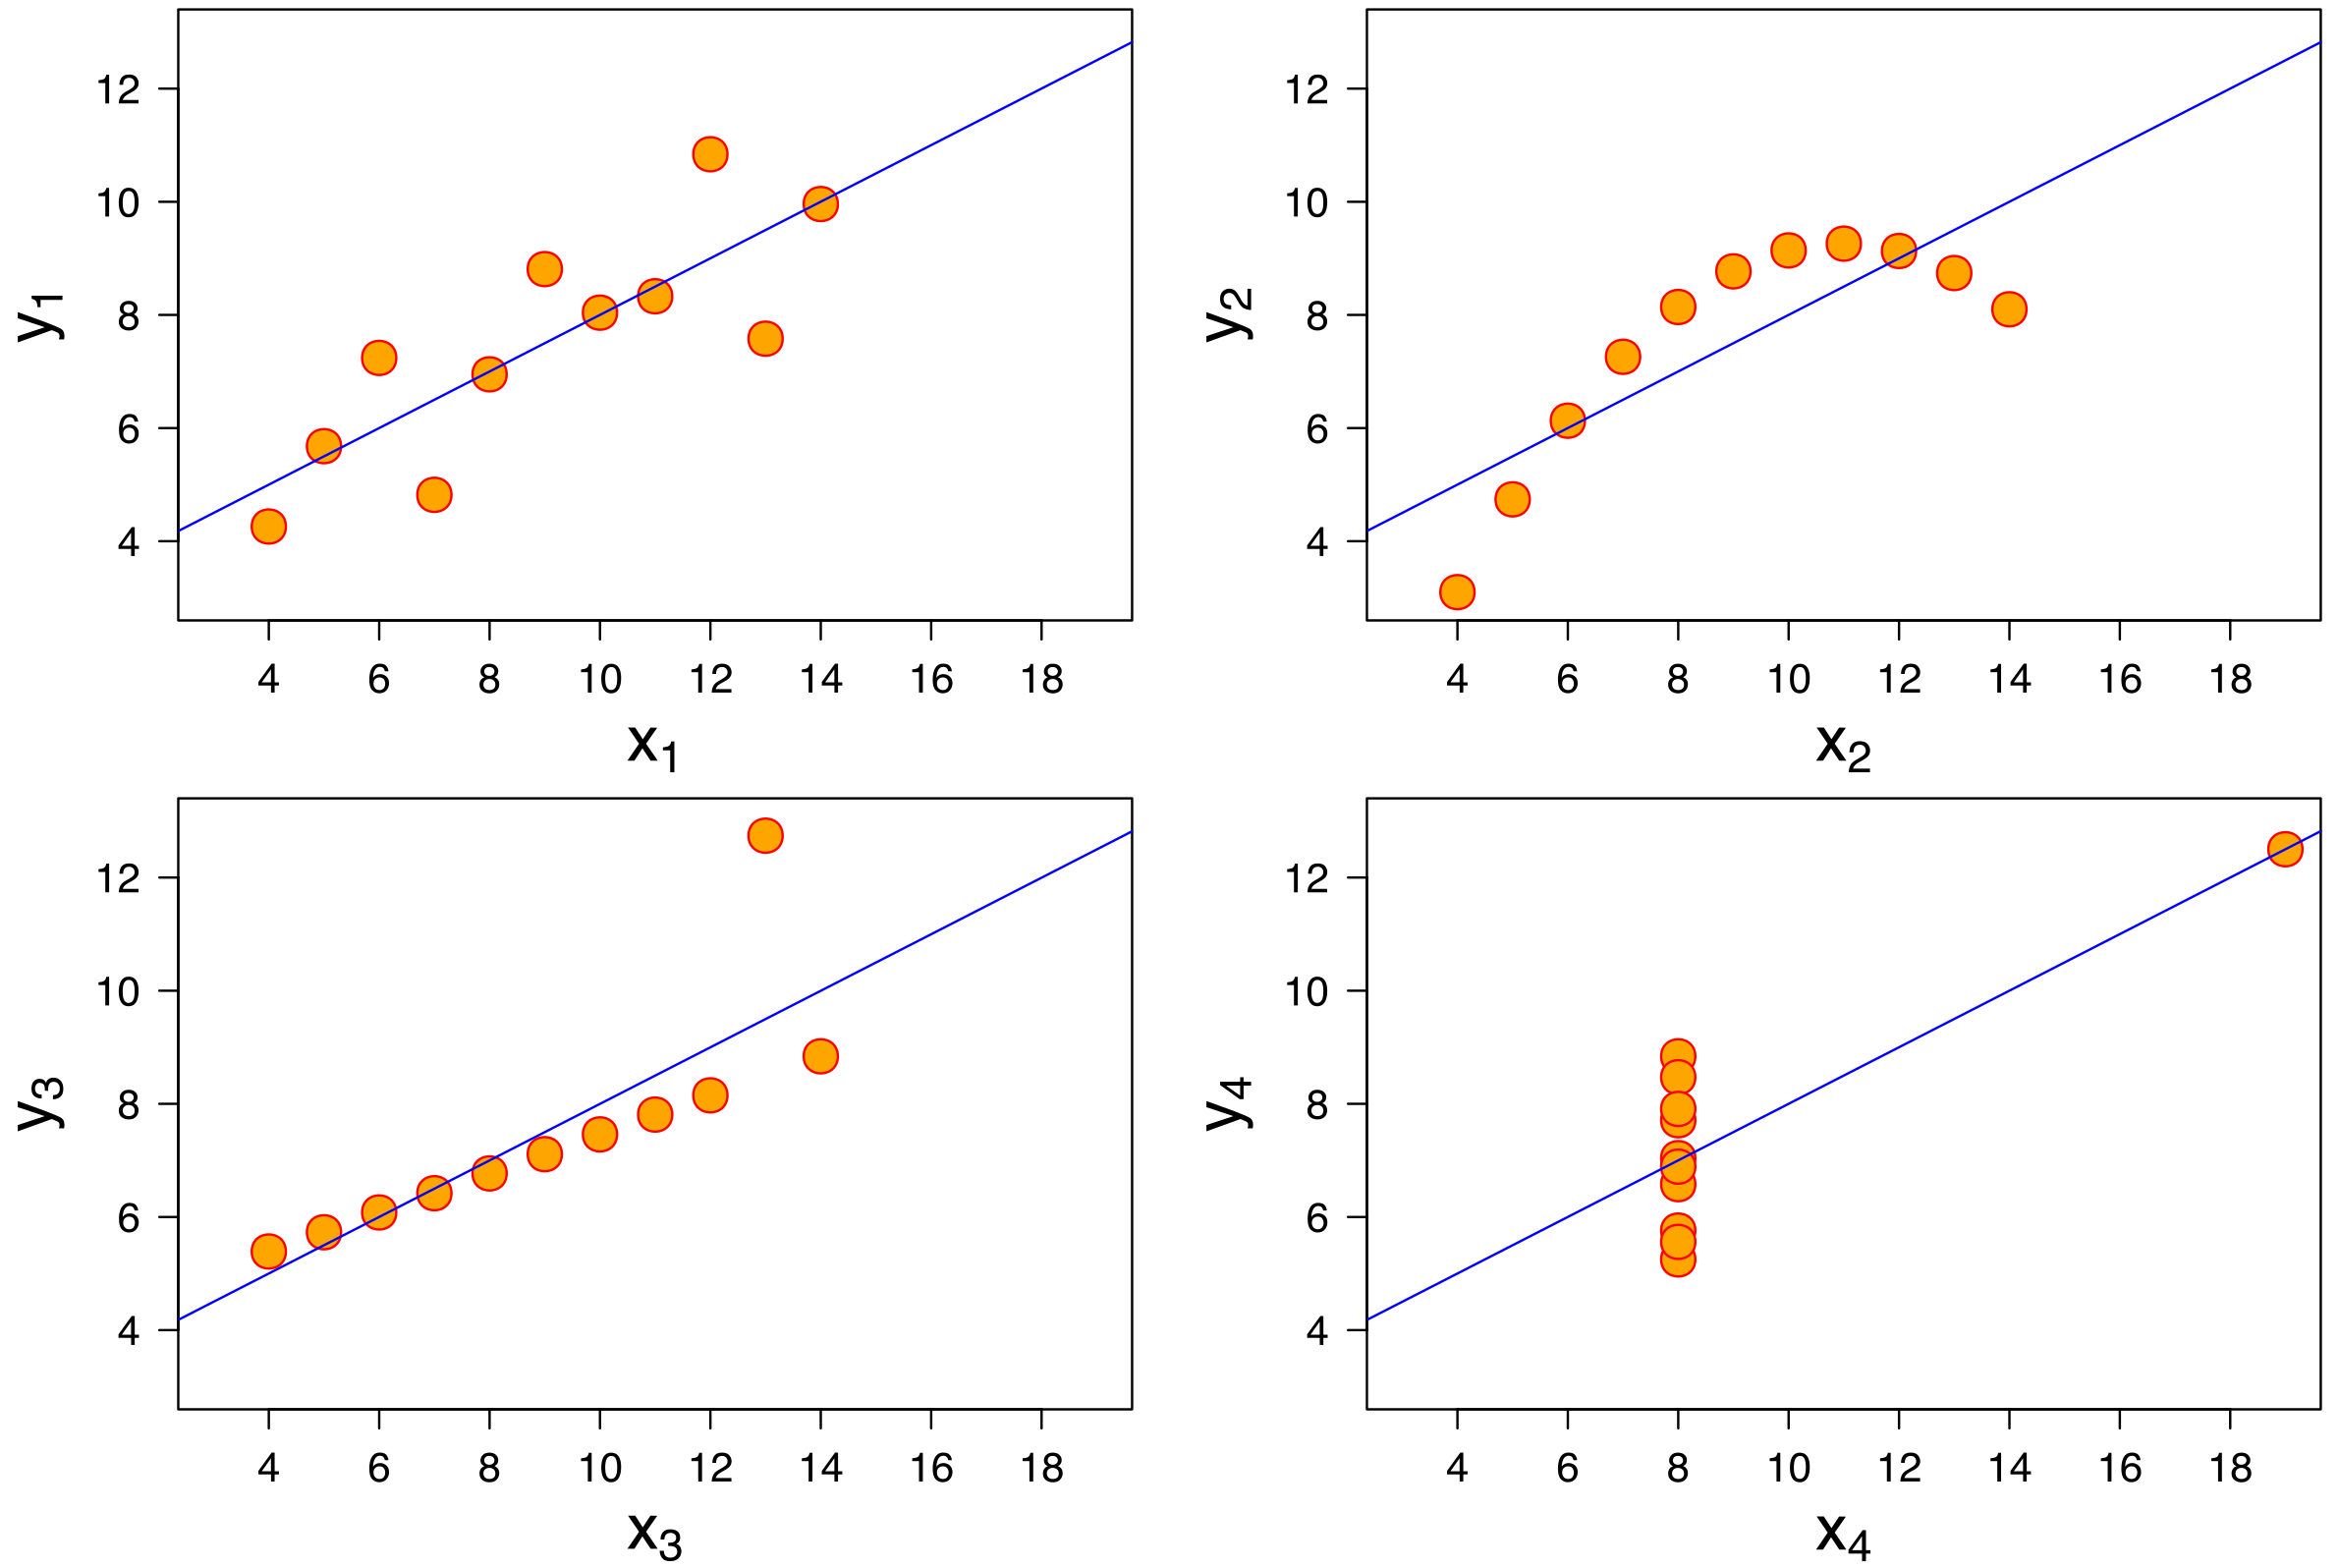
\includegraphics[width=0.9\linewidth]{ch03/anscombe.png}
    \caption{All four sets are identical when examined using simple summary statistics, but vary considerably when graphed. $\bar{x} = 9$, $\bar{y} = 7.50$, $s_x^2 = 11$, $s_y^2 = 4.125$, correlation $r = 0.816$, linear regression line $\hat{y} = 3.00 + 0.500x$, coefficient of determination $r^2 = 0.67$.}
    \label{fig:anscombe}
\end{figure}

\begin{figure}[ht!]
    \centering
    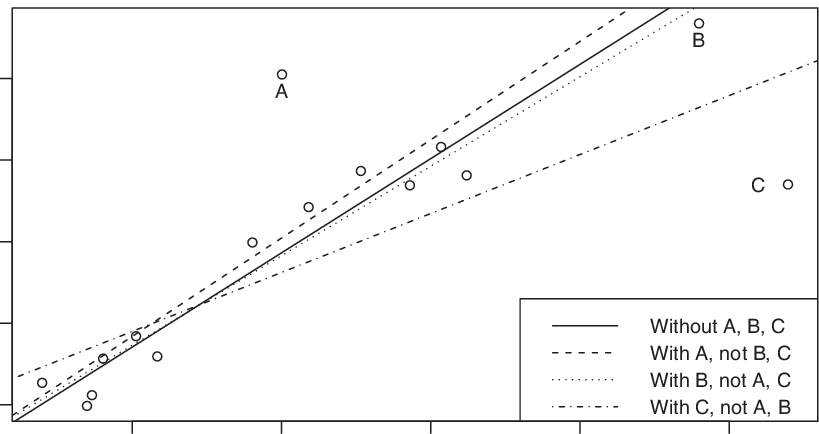
\includegraphics[width=0.6\linewidth]{ch03/regression-outlier.png}
    \caption{Outliers in regression are observations that fall far from the ``cloud'' of points. These points are especially important because they can have a strong influence on the least squares line.}
    \label{fig:regression-outlier}
\end{figure}

\subsubsection{Residual Plot}

A \textbf{residual plot} in effect turns the regression line horizontal. It magnifies the deviations of the points from the line, making it easier to see unusual observations and patterns.

\begin{definition}{Residual plot}{}
    A \textbf{residual plot} is a scatterplot of the residuals against the explanatory variable. Residual plots help us assess whether a linear model is appropriate.
\end{definition}

When an obvious curved pattern exists in a residual plot, the model we are using is not appropriate. Remember when we calculate a residual, we are calculating what is left over after subtracting the predicted value from the observed value:
\[
    \text{residual} = \text{observed $y$} - \text{predicted $y$}.
\]
Likewise, when we look at the form of a residual plot, we are looking at the form that is left over after subtracting the form of the model from the form of the association:
\[
    \text{form of residual plot}
    = \text{form of association}
    - \text{form of model}.
\]
When there is a leftover form in the residual plot, the form of the association and form of the model are not the same. However, if the form of the association and form of the model are the same, the residual plot should have no form, other than \textit{random scatter}.

\subsubsection{The Standard Deviation of the Residuals: $s$}

To assess how well the line fits all the data, we need to consider the residuals for each of the predictions we made, not just one. Using these residuals, we can estimate the ``typical'' prediction error when using the least-squares regression line. To do this, we calculate the standard deviation of the residuals.

\begin{definition}{Standard deviation of the residuals}{}
    If we use a least-squares line to predict the values of a response variable $y$ from an explanatory variable $x$, the \textbf{standard deviation of the residuals} ($s$) is given by
    \[
        s
        = \sqrt{\dfrac{\sum\text{residuals}^2}{n-2}}
        = \sqrt{\dfrac{\sum(y_i - \hat{y})^2}{n-2}}.
    \]
    This value gives the approximate size of a \textit{typical prediction error}, i.e., residual.
\end{definition}

\subsubsection{The Coefficient of Determination: $r^2$}

If we don't know the value for the additional explanatory variable, we can't use the regression line to make a prediction. What should we do? Our best strategy is to use the mean value of the response variable of the other points as our prediction. However, if we learn the value of the new explanatory variable $x$, then we could use the least-squares line to make prediction. How much better does the regression line do at prediction than simply using the average $\bar{y}$?

\begin{definition}{The coefficient of determination}{}
    The \textbf{coefficient of determination} $r^2$ is the fraction of the variation in the values of $y$ that is accounted for by the least-squares regression line of $y$ on $x$. We can calculate $r^2$ using the following formula:
    \[
        r^2 = 1 - \dfrac{\sum\text{residuals}^2}{\sum(y_i - \bar{y})^2}.
    \]
\end{definition}

If all the points fall directly on the least-squares line, the sum of squared residuals is 0 and $r^2 = 1$. Then all the variation in $y$ is accounted for by the linear relationship with $x$. Because the least-squares line yields the smallest possible sum of squared prediction errors, the sum of squared residuals can never be more than the sum of squared deviations from the mean of $y$. In the worst-case scenario, the least-squares line does no better at predicting $y$ than $y = \bar{y}$ does. Then the two sums of squares are the same and $r^2 = 0$.

It seems fairly remarkable that the coefficient of determination is actually the correlation squared. This fact provides an important connection between correlation and regression. When you see a correlation, square it to get a better feel for how well the least-squares line fits the data.

\clearpage

\section{Probability Fundamentals}

\paragraph{Chance process}
A {chance process} has outcomes that we cannot predict but that nonetheless have a regular distribution in very many repetitions. \textbf{The law of large numbers} says that the proportion of times that a particular outcome occurs in many repetitions will approach a single number. This long-run relative frequency of a chance outcome is its \textbf{probability}. A probability is a number between 0 (never occurs) and 1 (always occurs).

Probabilities describe only what happens in the long run. Short runs of random phenomena like tossing coins or shooting a basketball often don't look random to us because they do not show the regularity that emerges only in very many repetitions.

\paragraph{Simulation}
A {simulation} is an imitation of chance behavior, most often carried out with random numbers. To perform a simulation, follow the four-step process:
\begin{itemize}[font=\sffamily\bfseries, leftmargin=1.95cm, style=nextline, itemsep=0cm]
\item[State] Ask a question of interest about some chance process.
\item[Plan] Describe how to use a chance device to imitate one repetition of the process. Tell what you will record at the end of each repetition.
\item[Do] Perform many repetitions of the simulation.
\item[Conclude] Use the results of your simulation to answer the question of interest.
\end{itemize}

\subsection{Basic Probability Rules}

\paragraph{Sample space}
A \textbf{probability model} describes chance behavior by listing the possible outcomes in the \textbf{sample space} $S$ and giving the probability that each outcome occurs.

\paragraph{Events}
An \textbf{event} is a subset of the possible outcomes in the sample space. To find the probability that an event $A$ happens, $\pr(A)$, we can rely on some basic probability rules:

\begin{itemize}[style=nextline, itemsep=0cm]
\item For any event $A$, $0 \leq \pr(A) \leq 1$.
\item $\pr(S) = 1$, where $S$ is the sample space.
\item If all outcomes in the sample space are equally likely, then
    $$
        \pr(A) = \dfrac{
            \text{\# outcomes corresponding to event $A$}
        }{
            \text{\# outcomes in the sample space}
        }.
    $$
\end{itemize}

\subsection{Probability Involving Multiple Events}
A \textbf{two-way table} or a \textbf{Venn diagram} can be used to display the sample space for a chance process. Two-way tables and Venn diagrams can also be used to find probabilities involving events $A$ and $B$. For example, event $A \cup B$ ($A$ or $B$) consists of all outcomes in event $A$, event $B$, or both. Event $A \cap B$ ($A$ and $B$) consists of all outcomes in both $A$ and $B$.

\paragraph{Complement rule}
Event $A^C$ ($A$ not happen) consists of all outcomes not in event $A$, whose probability is given by
$$
    \pr\left( A^C \right) = 1 - \pr(A).
$$

\paragraph{Addition rule}
The general addition rule states that the probability of either A or B, or both, happens is
$$
    \pr(\text{$A$ or $B$})
    = \pr(A \cup B)
    = \pr(A) + \pr(B) - \pr(A \cap B).
$$
In the special case that $A$ and $B$ are \textit{mutually exclusive} (disjoint), i.e., they have no outcomes in common, the addition rule becomes
$$
    \pr(\text{$A$ or $B$})
    = \pr(A \cup B)
    = \pr(A) + \pr(B).
$$

\subsection{Conditional Probability}

\paragraph{Conditional probability}
If one event $B$ has happened, the chance that another event $A$ will happen is a \textbf{conditional probability}, denoted $\pr(A \mid B)$, which can be calculated by
$$
    \pr(A \mid B) = \dfrac{\pr(A \cap B)}{\pr(B)}.
$$

\paragraph{Multiplication rule}
The general multiplication rule states that the probability of events $A$ and $B$ occurring together is
$$
    \pr(\text{$A$ and $B$})
    = \pr(A \cap B)
    = \pr(A) \pr(B \mid A).
$$
In the special case of \textit{independent} events, the multiplication rule becomes
$$
    \pr(\text{$A$ and $B$})
    = \pr(A \cap B)
    = \pr(A) \pr(B).
$$

\paragraph{The law of total probability}
Let events $B_1, B_2, ..., B_n$ be a \textbf{partition} of the sample space, i.e., they are disjoint and their union is the entire sample space. Then
$$
    \pr(A) = \sum_{i=1}^{n} \pr(A \mid B_i) \pr(B_i).
$$

\paragraph{Bayes' theorem}
Bayes' theorem gives a way of \textit{inverting} conditions:
$$
    \pr(A \mid B)
    = \dfrac{\pr(B \mid A) \pr(A)}{\pr(B)},
$$
where
\begin{itemize}[style=nextline, itemsep=0cm]
\item $\pr(A \mid B)$ is the probability of event $A$ occurring given $B$ has already happened, a.k.a., the \textbf{posterior} of $A$ given $B$.
\item $\pr(B \mid A)$ is the probability of event $B$ occurring given $A$ has already happened.
\item $\pr(A)$ and $\pr(B)$ are the probabilities of observing $A$ and $B$ respectively without given any conditions, a.k.a., \textbf{marginal probability} or \textbf{prior probability}. They can often be found using the law of total probability.
\end{itemize}

\subsection{Mutually Exclusive Events vs. Independent Events}

\paragraph{Mutually exclusive events}
Events are \textbf{mutually exclusive} if the occurrence of one event excludes the occurrence of the other(s). Mutually exclusive events cannot happen at the same time. For example, when tossing a coin, the result can either be heads or tails but cannot be both.

\paragraph{Independent events}
Events are \textbf{independent} if the occurrence of one event does not influence (and is not influenced by) the occurrence of the other(s). For example, when tossing two coins, the result of one flip does not affect the result of the other. Formally, two events are independent iff one of the following equivalent statements holds:
\begin{align*}
    \pr(A \cap B) &= \pr(A) \pr(B) \\
    \pr(A \mid B) &= \pr(A) \\
    \pr(B \mid A) &= \pr(B) \\
\end{align*}

In a word, \textit{mutually exclusive events are not independent, and independent events are not mutually exclusive}.

\begin{table}[ht!]
    \centering
    \begin{tabular}{ccc}
        \toprule
        & Mutually exclusive & Independent \\
        \midrule
        $\pr(A \cap B)$ & $0$ & $\pr(A) \pr(B)$ \\
        $\pr(A \cup B)$ & $\pr(A) + \pr(B)$ & $\pr(A)+\pr(B)-\pr(A)\pr(B)$ \\
        $\pr(A \mid B)$ & $0$ & $\pr(A)$ \\
        $\pr\left(A \mid B^C\right)$ & $\dfrac{\pr(A)}{1-\pr(B)}$ & $\pr(A)$ \\
        \bottomrule
    \end{tabular}
\end{table}

\clearpage

\section{Random Variables}

\paragraph{Random variable} A random variable takes numerical values determined by the outcome of a chance process. The \textbf{probability distribution} of a random variable $X$ tells us what the possible values of $X$ are and how probabilities are assigned to those values. There are two types of random variables: discrete and continuous.
\begin{itemize}[font=\sffamily\bfseries, leftmargin=1.95cm, style=nextline, itemsep=0cm]
\item[Discrete] A discrete random variable has a \textit{fixed set of possible values} with gaps between them. The probability distribution assigns each of these values a probability between 0 and 1 such that the sum of all the probabilities is exactly 1. The probability of any event is the sum of the probabilities of all the values that make up the event.
\item[Continuous] A continuous random variable takes all values in some \textit{interval of numbers}. A density curve describes the probability distribution of a continuous random variable. The probability of any event is the area under the curve above the values that make up the event.
\end{itemize}

\paragraph{Expected value} Expected value (a.k.a., \textit{mean}, \textit{expectation}, or \textit{average}) is a weighted average of the possible outcomes of a random variable. Mathematically, if $x_1, x_2, ..., x_n$ are all of the distinct possible values that a discrete random variable $X$ can take, the expected value of $X$ is given by
$$
    \mu_X = \ev[X] = \sum_{i=1}^{n} x_i \pr(X=x_i).
$$

\paragraph{Linearity of expected value} For any random variables $X$ and $Y$, and constants $a$, $b$, and $c$,
$$
    \ev[aX + bY + c] = a\ev[X] + b\ev[Y] + c.
$$

\paragraph{Variance and standard deviation} For a random variable $X$, its variance $\delta_X^2$ is the \textit{average squared deviation} of the values of the variable from their mean; its standard deviation $\delta_X$ is the square root of the variance, measuring the typical distance of the values in the distribution from the mean. For a discrete random variable $X$,
\begin{align*}
    \delta_X^2 &= \var[X] = \sum_{i=1}^{n} (x_i - \mu_X)^2 \pr(X=x_i) \\
    \delta_X   &= \sqrt{\delta_X^2}
\end{align*}

\subsection{Transforming Random Variables}

\paragraph{Addition and subtraction} Adding a positive constant $a$ to (or subtracting $a$ from) a random variable increases (decreases) the mean of the random variable by $a$ but does not affect its standard deviation or the shape of its probability distribution.

\paragraph{Multiplication and division} Multiplying (dividing) a random variable by a positive constant $b$ multiplies (divides) the mean of the random variable by $b$ and the standard deviation by $b$ but does not change the shape of its probability distribution.

\begin{table}[ht!]
    \centering
    \begin{tabular}{cccc}
        \toprule
        & \makecell{Center and location\\\textit{Mean, median,}\\\textit{quartiles, percentiles}}
        & \makecell{Spread\\\textit{range, IQR,}\\\textit{standard deviation}}
        & Shape \\
        \midrule
        $X + a$ & increased by $a$ & No change & No change \\
        $X - a$ & decreased by $a$ & No change & No change \\
        $bX$    & multiplied by $b$ & multiplied by $b$ & No change \\
        $X/b$   & divided by $b$ & divided by $b$ & No change \\
        \bottomrule
    \end{tabular}
\end{table}

\paragraph{Linear transformation} A linear transformation of a random variable involves adding or subtracting a constant $a$, multiplying or dividing by a constant $b$, or both. We can write a linear transformation of the random variable $X$ in the form $Y = a + bX$. The shape, center, and spread of the probability distribution of $Y$ are as follows:
\begin{itemize}[font=\sffamily\bfseries, leftmargin=1.95cm, style=nextline, itemsep=0cm]
\item[Shape] Same as the probability distribution of $X$ if $b > 0$
\item[Center] $\mu_Y = a + b\mu_X$
\item[Spread] $\delta_Y = |b| \delta_X$
\end{itemize}

\subsection{Combining Random Variables}

\paragraph{Mean of combined random variables} If $X$ and $Y$ are \textit{any} two random variables,
$$
    \mu_{X \pm Y} = \mu_X \pm \mu_Y.
$$

\paragraph{Variance of combined random variables} If $X$ and $Y$ are two \textit{independent} random variables,
$$
    \delta^2_{X \pm Y} = \mu_X + \mu_Y.
$$
Note that the variance of either the sum or the difference of two independent variables is \textit{always} the sum of their variances.

\paragraph{Combined normal random variables} Let $X$ and $Y$ be independent random variables that are normally distributed, then their sum is also normally distributed, i.e., if
$$
    X \sim N\left(\mu_X, \delta_X^2\right), \quad
    Y \sim N\left(\mu_Y, \delta_Y^2\right), \quad
    Z = X + Y,
$$
then
$$
    Z \sim N\left(\mu_X + \mu_Y, \delta_X^2 + \delta_Y^2\right)
$$

\subsection{Binomial Distribution}

\paragraph{Binomial coefficient} The binomial coefficient counts the number of ways $k$ successes can be arranged among $n$ trials, calculated by
$$
    {n \choose k} = \dfrac{n!}{k!(n-k)!},
$$
where the factorial of $n$ is
$$
    n! = n(n-1)(n-2) \cdots (3)(2)(1),
$$
for positive whole numbers $n$ and $0! = 1$.

\paragraph{Binomial settings} A binomial setting consists of $n$ independent trails of the same chance process, each resulting in a success or a failure, with probability of success $p$ on each trial. The count $X$ of successes is a \textbf{binomial random variable}. Its probability distribution is a \textbf{binomial distribution}.

\paragraph{Binomial distribution} If $X$ has the binomial distribution with parameters $n$ and $p$, i.e., $X \sim \mathrm{Binomial}(n, p)$, the possible values of $X$ are the whole numbers $0, 1, ..., n$. Its probability mass function (pmf), mean, and variance are given by
\begin{itemize}[font=\sffamily\bfseries, leftmargin=1.95cm, style=nextline, itemsep=0cm]
\item[pmf] $\pr(X=k) = {n \choose k} p^k (1-p)^{n-k}$
\item[Mean] $\mu_X = np$
\item[Variance] $\delta_X^2 = np(1-p)$
\end{itemize}

\paragraph{Shape of binomial distribution} The shape of the binomial distribution is directly controlled by $n$ -- the number of independent trials, and $p$ -- the probability of success.
\begin{itemize}[font=\sffamily\bfseries, leftmargin=3cm, style=nextline, itemsep=0cm]
\item[Small $\mathbf{p}$, small $\mathbf{n}$] The binomial distribution is \textit{skewed right}, i.e., the bulk of the probability falls in the smaller numbers $0, 1, 2, ...$, and the distribution tails off to the right. See Figure \ref{fig:binomial} ($n=15, p=0.1$) and ($n=15, p=0.2$).
\item[Large $\mathbf{p}$, small $\mathbf{n}$] The binomial distribution is \textit{skewed left}, i.e., the bulk of the probability falls in the smaller numbers $n, n-1, n-2, ...$, and the distribution tails off to the left. See Figure \ref{fig:binomial} ($n=15, p=0.8$) and ($n=15, p=0.9$).
\item[$\mathbf{p=0.5}$, all $\mathbf{n}$] The binomial distribution is \textit{symmetric}. See Figure \ref{fig:binomial} ($n=15, p=0.5$) and ($n=40, p=0.5$).
\item[All $\mathbf{p}$, large $\mathbf{n}$] The binomial distribution \textit{approaches symmetry}. For example, if $p=0.2$ and $n$ is small, we'd expect the binomial distribution to be skewed to the right. For large $n$, however, the distribution is \textit{nearly symmetric}. See Figure \ref{fig:binomial} ($n=40, p=0.1$), ($n=40, p=0.2$), ($n=40, p=0.8$), ($n=40, p=0.9$).
\end{itemize}

\begin{figure}[ht!]
    \centering
    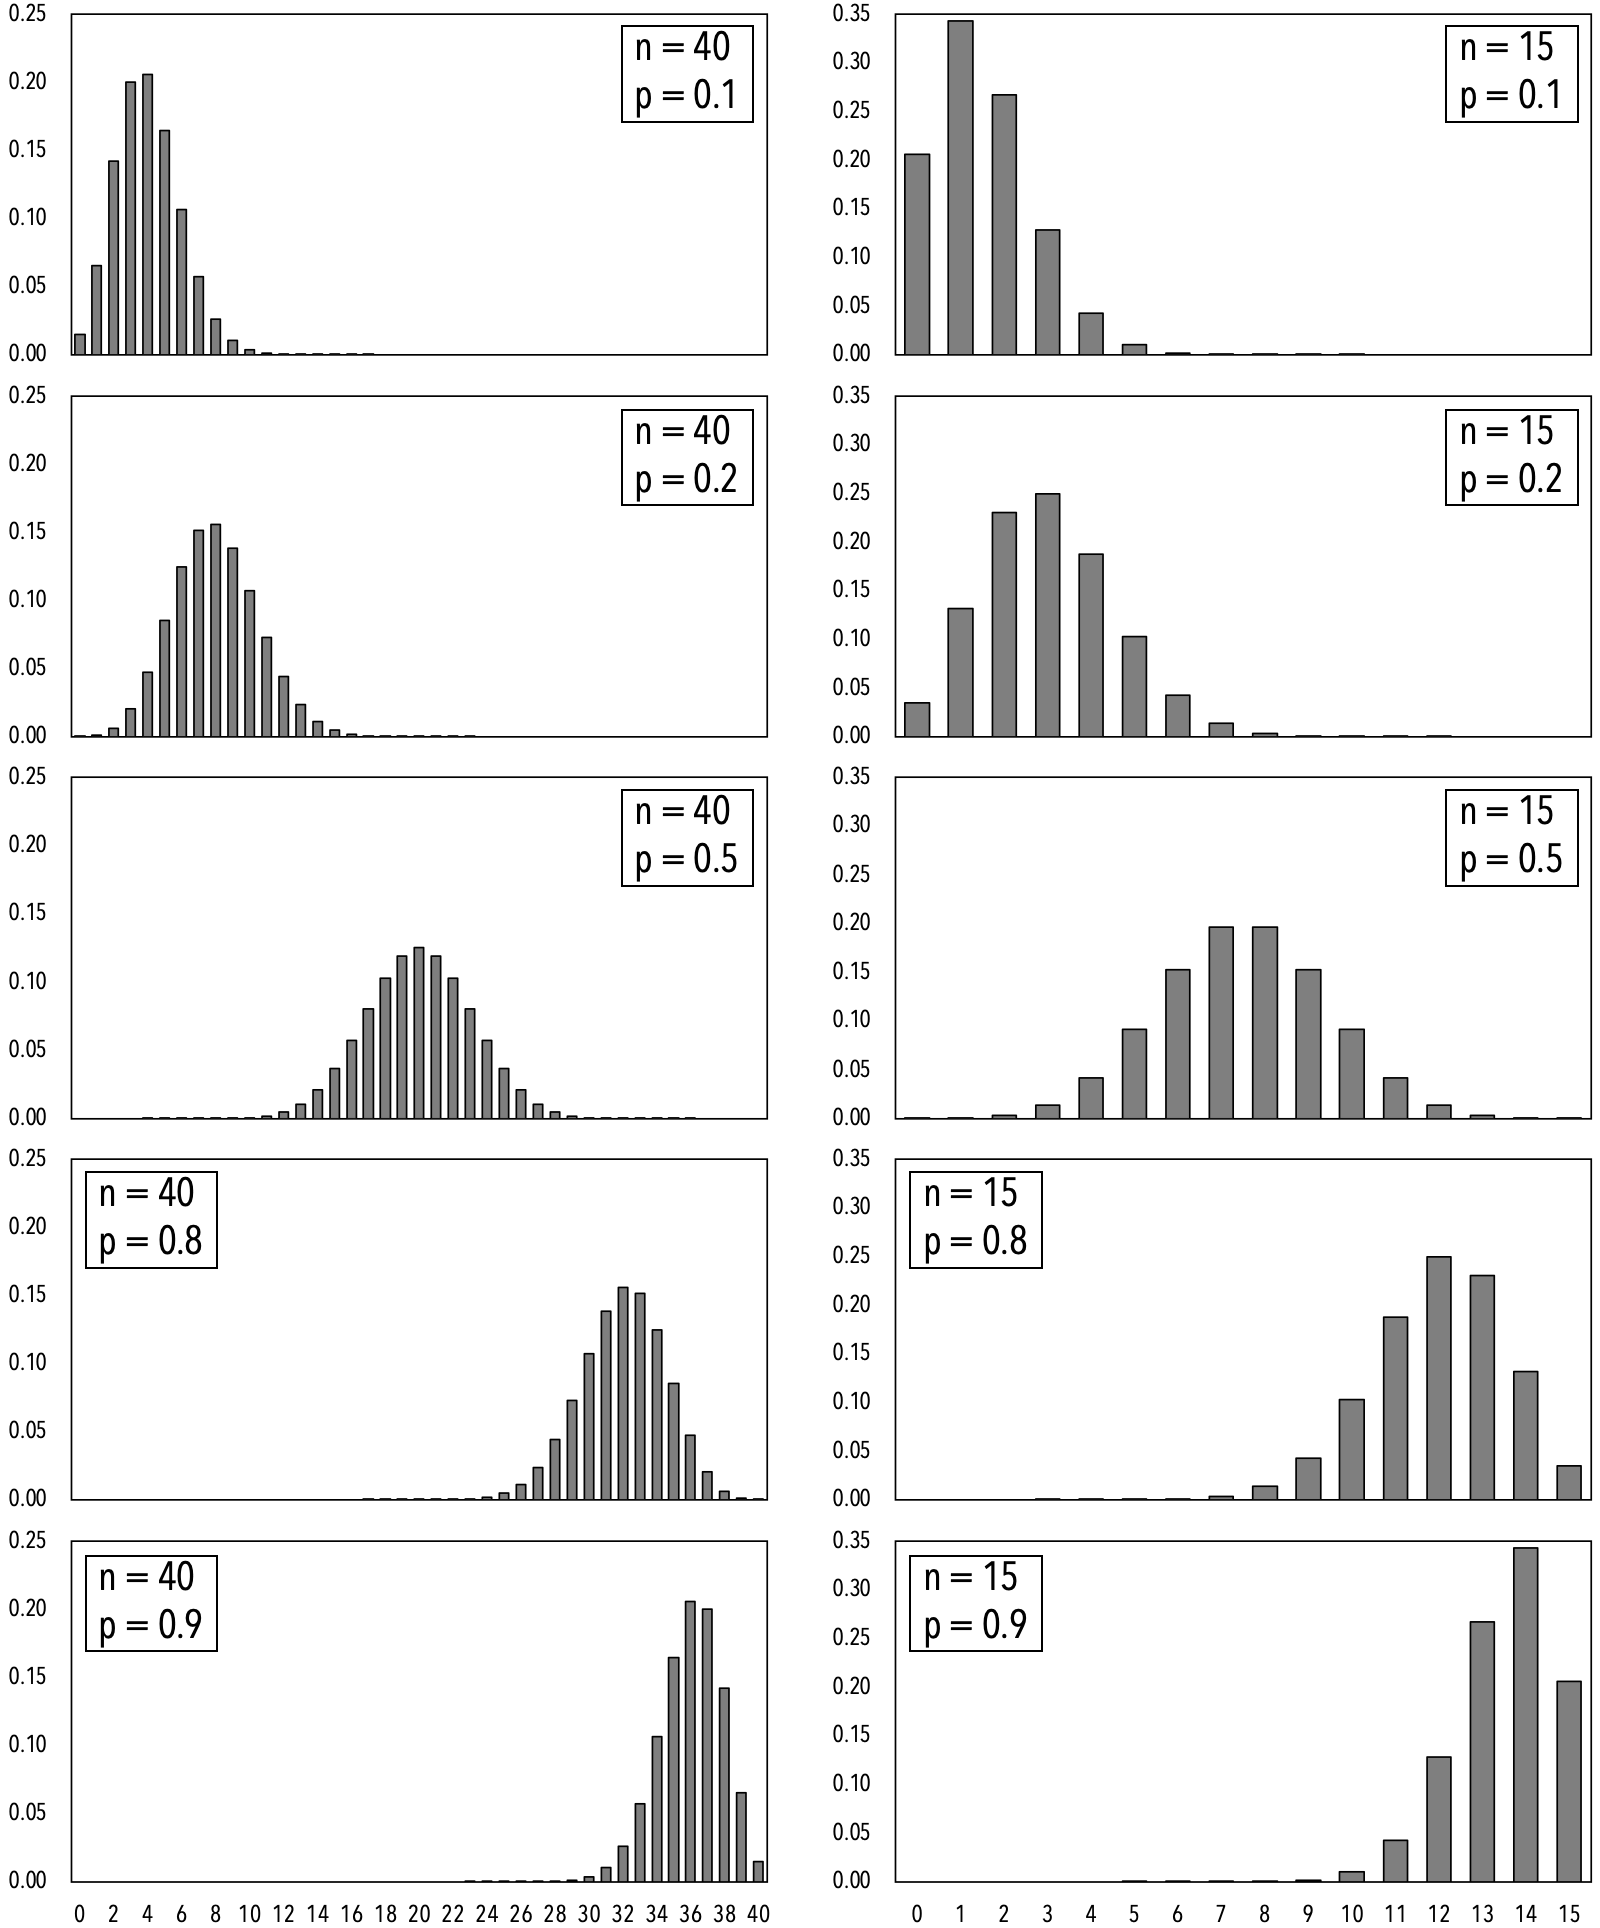
\includegraphics[width=\linewidth]{ch06/binomial.png}
    \caption{Comparison of binomial distribution of different parameters.}
    \label{fig:binomial}
\end{figure}

\subsection{Geometric Distribution}

\paragraph{Geometric settings} A geometric setting consists of repeated trials of the same chance process in which the probability $p$ of success is the same on each trial, and the goal is to count the number of trials it takes to get one success. If $Y$ is the number of trials required to obtain the first success, then $Y$ is a geometric random variable. Its probability distribution is called a geometric distribution.

\paragraph{Geometric distribution} If $Y$ has the geometric distribution with probability of success $p$, i.e., $Y \sim \mathrm{Geometric}(p)$, the possible values of $Y$ are the positive integers $1, 2, 3, ...$. Its probability mass function (pmf), mean, and variance are given by
\begin{itemize}[font=\sffamily\bfseries, leftmargin=1.95cm, style=nextline, itemsep=0cm]
\item[pmf] $\pr(Y=k) = (1-p)^{k-1}p$
\item[Mean] $\mu_Y = 1/p$
\item[Variance] $\delta_Y^2 = (1-p)/p^2$
\end{itemize}

\paragraph{Shape of binomial distribution} The shape of the geometric distribution is directly controlled by $p$ -- the probability of success. The larger the $p$, the steeper the function in the beginning. Note that the function is \textit{monotonically decreasing}.

\begin{figure}[ht!]
    \centering
    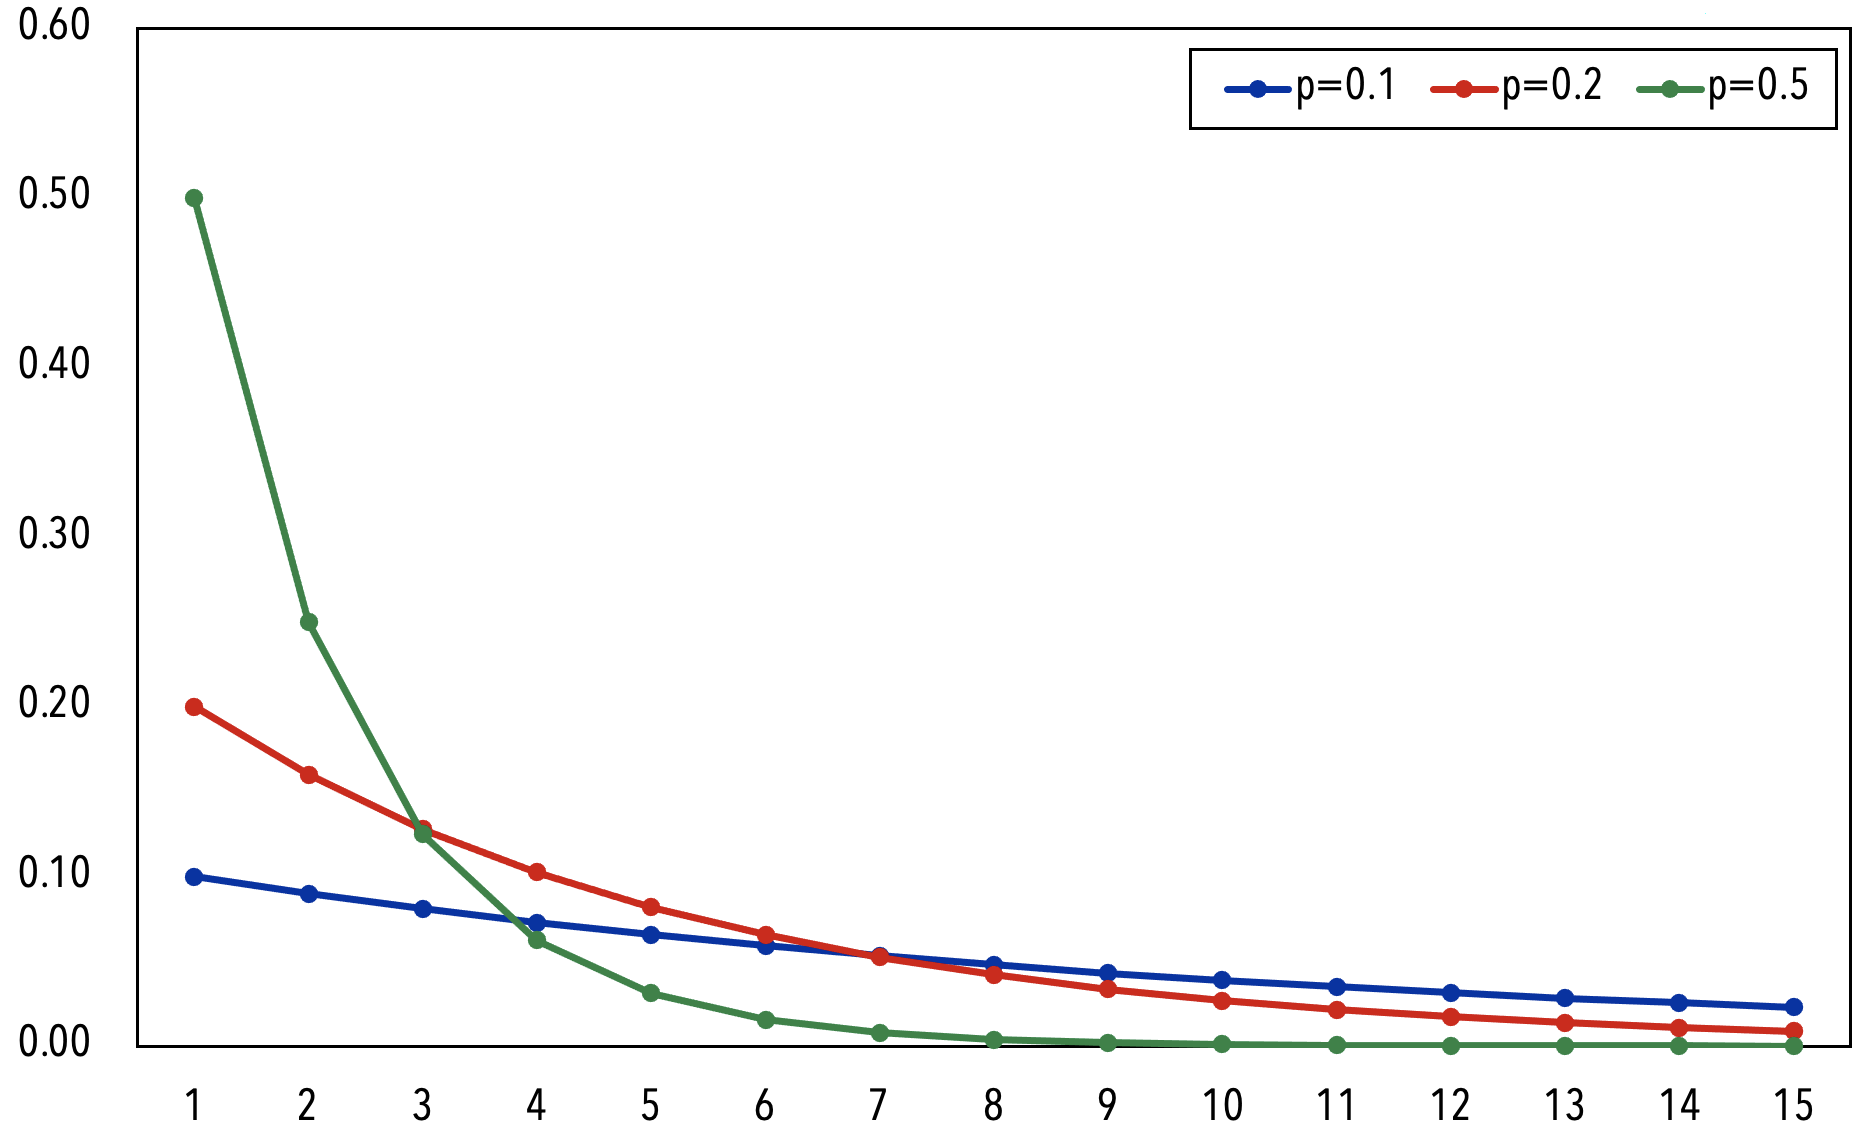
\includegraphics[width=0.8\linewidth]{ch06/geometric.png}
    \caption{Comparison of geometric distribution of different parameters.}
    \label{fig:geometric}
\end{figure}

\clearpage

\end{document}
